\documentclass[final]{beamer}
\mode<presentation>{\usetheme{default}}
\usepackage[size=a0,scale=1.3,orientation=portrait]{beamerposter}
\usepackage[utf8]{inputenc}
\usepackage[english]{babel}
\usepackage{amsmath,amsthm,amssymb}
\usepackage{graphicx}
\usepackage{tcolorbox}
\usepackage{qrcode}

% Color definitions
\definecolor{headerred}{RGB}{153,0,51}
\definecolor{darkred}{RGB}{120,0,40}

% Custom tcolorbox styles
\tcbset{
    mybox/.style={
        colback=white,
        colframe=headerred,
        fonttitle=\bfseries\Large,
        coltitle=white,
        colbacktitle=headerred,
        enhanced,
        attach boxed title to top left={yshift=-2mm, xshift=5mm},
        boxed title style={sharp corners},
        sharp corners,
        boxrule=1.5pt,
        top=5pt,
        bottom=5pt,
        left=8pt,
        right=8pt
    }
}

\setbeamertemplate{navigation symbols}{}
\setbeamertemplate{headline}{}

\begin{document}
\begin{frame}[t]

% Header
\begin{tcolorbox}[colback=white,colframe=headerred,boxrule=2pt,arc=0pt,
    left=10pt,right=10pt,top=5pt,bottom=5pt]
\begin{minipage}{0.12\linewidth}
\centering
\end{minipage}
\hfill
\begin{minipage}{1.0\linewidth}
\centering
{\fontsize{65}{78}\selectfont\textbf{Empirical Properties of Asset Returns}}\\[0.3cm]
{\fontsize{48}{58}\selectfont Stylized Facts and Statistical Issues}\\[0.2cm]
{\Large\textbf{Author:} Rama Cont | École Polytechnique, France}
\end{minipage}
\end{tcolorbox}

\vspace{0.6cm}

\begin{columns}[t]

% ============= LEFT COLUMN =============
\begin{column}{.48\linewidth}

% ABSTRACT
\begin{tcolorbox}[mybox, title=Abstract]
\large

We present a set of stylized empirical facts emerging from the statistical
analysis of price variations in various types of financial markets. We first
discuss some general issues common to all statistical studies of financial time
series. Various statistical properties of asset returns are then described:
distributional properties, tail properties and extreme fluctuations, pathwise
regularity, linear and nonlinear dependence of returns in time and across
stocks. Our description emphasizes properties common to a wide variety of
markets and instruments. We then show how these statistical properties
invalidate many of the common statistical approaches used to study financial
data sets and examine some of the statistical problems encountered in each
case.

\end{tcolorbox}

\vspace{0.5cm}

% KEYWORDS
\begin{tcolorbox}[mybox, title=Keywords]
\large
\textbf{Stylized facts} $\bullet$ \textbf{Heavy tails} $\bullet$ \textbf{Volatility clustering} $\bullet$ \textbf{Long-range dependence} $\bullet$ \textbf{Risk management}
\end{tcolorbox}

\vspace{0.5cm}

% MOTIVATION
\begin{tcolorbox}[mybox, title=Motivation]
\large
Although statistical properties of financial time series have been studied for decades, the emergence of high-frequency data poses a critical challenge to researchers in synthetically and meaningfully capturing the properties of this massive data set.
To address this challenge, a set of universal properties common across different markets have been identified by independent studies and are classified as \textbf{stylized facts}.
These stylized facts, such as \textbf{heavy tails} and \textbf{non-linear dependence}, fundamentally invalidate many of the common statistical approaches used to study financial data.
Our goal is to provide a pedagogical overview of these empirical properties, focusing on the data's characteristics and examining the resulting statistical issues encountered during real financial analysis.

% Despite different assets being influenced by different events, price series exhibit remarkably similar statistical properties.

% \vspace{0.3cm}
% \textbf{Question:} What common properties exist across different financial instruments, markets, and time periods?

% \vspace{0.3cm}
% These \textbf{stylized facts} constrain any realistic stochastic model.
\end{tcolorbox}

\vspace{0.5cm}

% PROBLEM
\begin{tcolorbox}[mybox, title=Problem Statement]
\large
\textbf{Traditional assumptions:}
\begin{itemize}
\item Normal distribution
\item Independent increments  
\item Constant volatility
\end{itemize}

\vspace{0.2cm}
\textbf{Reality:} Data systematically violates these!

\vspace{0.2cm}
\textbf{Objective:} Document model-free properties common across markets, robust across time, and constraining enough to rule out inadequate models.
\end{tcolorbox}

\vspace{0.5cm}

% HEAVY TAILS
\begin{tcolorbox}[mybox, title=Heavy Tails Distribution]
\begin{center}
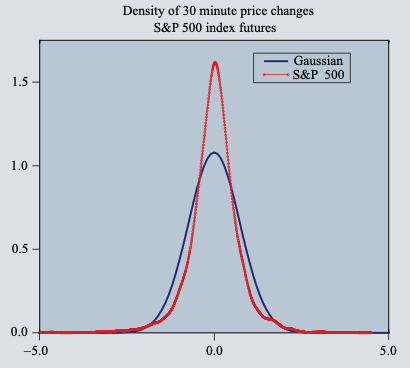
\includegraphics[width=0.98\linewidth,height=18cm,keepaspectratio]{figure2_density.png}
\end{center}
\vspace{0.3cm}
\large
Returns display \textbf{power-law tails} with $\alpha \in [2,5]$. Excludes both stable laws and normal distribution. Consistently heavier than Gaussian.
\end{tcolorbox}

\vspace{0.5cm}



\end{column}

% ============= RIGHT COLUMN =============
\begin{column}{.48\linewidth}


  % AUTOCORRELATION
\begin{tcolorbox}[mybox, title=Linear Autocorrelations]
\begin{center}
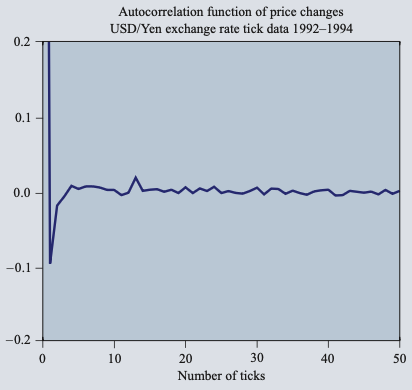
\includegraphics[width=0.95\linewidth,height=18cm,keepaspectratio]{figure6_autocorr.png}
\end{center}
\vspace{0.3cm}
\large
Returns are \textbf{insignificant} except at very short scales ($<$20 min). Supports efficient markets but does NOT imply independence.
\end{tcolorbox}


% % VOLATILITY CLUSTERING
% \begin{tcolorbox}[mybox, title=Volatility Clustering]
% \begin{center}
% 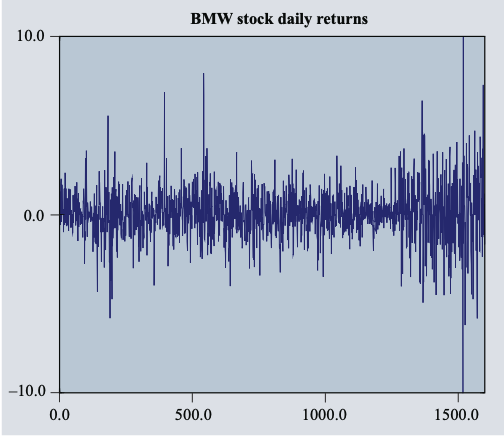
\includegraphics[width=0.95\linewidth,height=18cm,keepaspectratio]{figure1_bmw.png}
% \end{center}
% \vspace{0.3cm}
% \large
% \textbf{Large variations cluster in time.} Autocorrelation decays as: 
% $$C_\alpha(\tau) \sim A/\tau^\beta, \quad \beta \in [0.2, 0.4]$$

% Sign of \textbf{long-range dependence} in volatility.
% \end{tcolorbox}

\vspace{0.5cm}

% NONLINEAR
\begin{tcolorbox}[mybox, title=Nonlinear Correlations]
\begin{center}
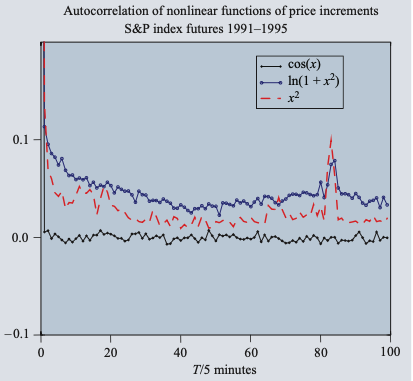
\includegraphics[width=0.95\linewidth,height=18cm,keepaspectratio]{figure8_nonlinear.png}
\end{center}
\vspace{0.3cm}
\large
Absolute/squared returns show strong persistence over days/weeks.
\end{tcolorbox}

\vspace{0.5cm}

% 11 STYLIZED FACTS
\begin{tcolorbox}[mybox, title=The 11 Stylized Facts]
\large
\begin{enumerate}
\item Absence of autocorrelations
\item Heavy tails % ($\alpha \in [2,5]$)
\item Gain/loss asymmetry
\item Aggregational Gaussianity
\item Intermittency
\item Volatility clustering
\item Conditional heavy tails
\item Slow decay of volatility correlations
\item Leverage effect
\item Volume/volatility correlation
\item Asymmetry in time scales
\end{enumerate}

% \vspace{0.2cm}
% Most models fail to reproduce all features simultaneously.
\end{tcolorbox}

\vspace{0.5cm}

% RESULTS/CONCLUSIONS
\begin{tcolorbox}[mybox, title=Results \& Conclusions]
\large
\begin{itemize}
\item Facts emerge \textbf{consistently} across markets, instruments, time periods
\item Heavy tails and clustering require \textbf{fundamental departure} from classical assumptions
\item Properties qualitatively stable; quantitative estimates challenging
\item Critical for \textbf{risk management} and VaR calculations
\end{itemize}
\end{tcolorbox}


\vspace{0.5cm}

% Acknowledgments
\begin{tcolorbox}[mybox, title=Acknowledgments]
\large
The author thanks Rokhsaneh Ghandi for constant encouragement and Doyne Farmer for many helpful comments on this
manuscript. This work has been supported by the CNRS Research Program on Quantitative Methods in Financial Modeling (FIQUAM).

\end{tcolorbox}

\end{column}
\end{columns}

\vspace{0.6cm}

% FOOTER
\begin{tcolorbox}[colback=white,colframe=headerred,boxrule=2pt,arc=0pt,
    left=10pt,right=10pt,top=5pt,bottom=5pt]
\begin{minipage}{0.7\linewidth}
\large
\textbf{Publication:} Quantitative Finance, Vol. 1 (2001), pp. 223--236 | \textbf{DOI:} 10.1080/713665670\\
\textbf{Acknowledgement:} Research supported by CNRS FIQUAM program
\end{minipage}
\hfill
\begin{minipage}{0.25\linewidth}
\centering
\qrcode[height=3cm]{https://doi.org/10.1080/713665670}\\
{\small Scan for paper}
\end{minipage}
\end{tcolorbox}

\end{frame}
\end{document}